\section{问题三的模型建立与求解}

\subsection{光伏预报数据的插值与时间匹配}

附件 3 提供 2025 年全年每天 0:00、6:00、12:00、18:00 四个发布时点、每次发布未来 24 个整点的光伏发电功率预报，共 $365\times4\times24$ 条记录。设发布时点为 $\tau\in\{0,6,12,18\}$，字段``预报 $k$ 小时''对应发布时间之后第 $k$ 个整点。以发布时刻已经观测到的实际光伏功率为左端点，与未来 24 个整点预报一起构成插值节点，分段线性插值到 10 分钟网格后乘以 $\Delta t = 1/6$ h，得到 10 分钟尺度的光伏电量预测：

\begin{equation}
  \widehat{P}^{(\tau)}_d(t) = \frac{1}{6}\,\mathrm{interp}\left(\tau,\, t\right),
  \label{eq:q3_pv}
\end{equation}

式中：$\tau$ 为预报的发布时点；$\widehat{P}^{(\tau)}_d(t)$ 为计划日 $d$、时段 $t$ 由时点 $\tau$ 的预报生成的光伏电量预测（kWh）；$\mathrm{interp}(\cdot)$ 为分段线性插值的功率结果（kW）。

以附件 2 的时刻列作为执行边界：6:00 的更新只能修改结束时刻晚于 6:00 的时段，12:00 与 18:00 同理。日内不更新负荷预测，因为附件 3 只提供光伏预报，负荷仍沿用问题二的周周期加权平均预测。

\subsection{发布时间匹配的联合残差场景}

问题三的联合残差场景需在每个发布时点分别构造。对历史日 $r$ 与发布时点 $\tau$，归档当日在该时点实际发出的样本外残差：

\begin{equation}
  e^L_r(t) = L_r(t) - \widehat{L}_r(t),
  \qquad
  e^{P,\tau}_r(t) = P_r(t) - \widehat{P}^{(\tau)}_r(t),
  \label{eq:q3_residual}
\end{equation}

式中：$e^L_r(t)$ 为负荷预测残差（kWh）；$e^{P,\tau}_r(t)$ 为由时点 $\tau$ 预报生成的光伏预测残差（kWh）。

在计划日 $d$ 的发布时点 $\tau$，只允许使用 $r<d$ 且实际值已全部揭晓的完整同日残差块，历史日权重与问题二一致：

\begin{equation}
  \omega_{d,r} = 0.98^{\,d-r}\left[\,1 + \mathbf{1}\{\operatorname{weekday}(d)=\operatorname{weekday}(r)\}\,\right].
  \label{eq:q3_weight}
\end{equation}

将权重归一化后有放回抽取 100 次，取经验频数为场景概率；完全相同的重复历史日场景在实现中合并并按出现频数赋权，这与保留 100 份重复变量严格等价，但显著降低了混合整数规划的规模。场景电量为

\begin{equation}
  L^{(\tau)}_{d,s}(t) = \max\{\widehat{L}_d(t) + e^L_s(t),\ 0\},
  \qquad
  P^{(\tau)}_{d,s}(t) = \max\{\widehat{P}^{(\tau)}_d(t) + e^{P,\tau}_s(t),\ 0\},
  \label{eq:q3_scenario}
\end{equation}

式中：$L^{(\tau)}_{d,s}(t)$ 与 $P^{(\tau)}_{d,s}(t)$ 分别为时点 $\tau$ 下、场景 $s$、时段 $t$ 的负荷电量与光伏电量（kWh）；光伏场景上界只使用当前发布时点以前已经观测到的最大光伏电量。

\subsection{0:00 原计划模型}

0:00 原计划模型与问题二完全一致：场景电量平衡同式~\eqref{eq:q2_balance}，储能状态递推与容量边界同式~\eqref{eq:q2_soc}，充放电互斥同式~\eqref{eq:q2_mutex}，终端软区间同式~\eqref{eq:q2_lower} 与式~\eqref{eq:q2_upper}（其中季节基准 $B_d^{\mathrm{season}}$ 与风险调整量 $\delta_d$ 由式~\eqref{eq:q2_season}、式~\eqref{eq:q2_riskadj} 给出）。区别只有一处：光伏场景改由附件 3 的预报生成，即式~\eqref{eq:q2_balance} 中的 $P_{d,s}(t)$ 取 $P^{(0)}_{d,s}(t)$。0:00 的目标函数为

\begin{equation}
  \min\left\{
    \sum_t \lambda(t) G_d(t)
    + \sum_s \pi_s \sum_t 5\lambda(t) H_{d,s}(t)
    + 1.1250\,\bigl(R_d + X_d\bigr)
  \right\},
  \label{eq:q3_obj0}
\end{equation}

式中：三项依次为计划购电费、期望紧急购电费与终端偏离惩罚（元），其含义与式~\eqref{eq:q2_obj} 一致。

\subsection{日内滚动调整模型}

对发布时点 $\tau \in \{6,12,18\}$，设重新优化后的购电量为 $A^{(\tau)}(t)$，相对 0:00 原计划的调整量为

\begin{equation}
  A^{(\tau)}(t) - G(t) = U^{(\tau)}(t) - V^{(\tau)}(t),
  \qquad
  A^{(\tau)}(t),\,U^{(\tau)}(t),\,V^{(\tau)}(t) \ge 0,
  \label{eq:q3_adjust}
\end{equation}

式中：$A^{(\tau)}(t)$ 为调整后购电量（kWh）；$U^{(\tau)}(t)$ 与 $V^{(\tau)}(t)$ 分别为相对原计划的上调量与下调量（kWh），二者是与终端偏离量 $R_d$、$X_d$ 无关的另一组变量。采用净结算口径：上调部分按 1.5 倍电价计费，下调取消部分按 50\% 电价承担违约费用，即时段结算费为

\begin{equation}
  F_t^{\mathrm{sch}} = \lambda(t)G(t) + 1.5\lambda(t)U^{(\tau)}(t) - 0.5\lambda(t)V^{(\tau)}(t),
  \label{eq:q3_schedule_cost}
\end{equation}

由于同一时段同时上调和下调只会增加费用，最优解中二者不会并存。若把下调理解为``计划量全额付费并另加 50\% 违约费''，下调的边际成本将由 0.5 倍电价升至 1.5 倍电价，滚动调整的幅度会明显减小，日内更新的价值会被低估。

剩余时域 $\mathcal T_\tau$ 上的场景电量平衡为

\begin{equation}
  A^{(\tau)}(t) + H^{(\tau)}_s(t) + P^{(\tau)}_s(t) + D^{(\tau)}(t)
  = L_s(t) + C^{(\tau)}(t) + W^{(\tau)}_s(t),
  \qquad t \in \mathcal T_\tau,
  \label{eq:q3_rolling_balance}
\end{equation}

式中：$\mathcal T_\tau$ 为发布时点 $\tau$ 之后尚未执行的时段集合。储能约束与 0:00 模型相同，但初始储电量改为当前实际已执行的储电量。去掉式~\eqref{eq:q3_schedule_cost} 中不随决策变化的常数项 $\sum_t\lambda(t)G(t)$ 后，滚动优化的目标函数为

\begin{equation}
  \begin{aligned}
    \min\Biggl\{
      &\sum_{t\in\mathcal T_\tau}\left[1.5\lambda(t)U^{(\tau)}(t) - 0.5\lambda(t)V^{(\tau)}(t)\right] \\
      &\quad + \sum_s \pi_s \sum_{t\in\mathcal T_\tau} 5\lambda(t) H_s(t)
      + 1.1250\,\bigl(R_d^{(\tau)} + X_d^{(\tau)}\bigr)\Biggr\}.
  \end{aligned}
  \label{eq:q3_objroll}
\end{equation}

式中：$R_d^{(\tau)}$ 与 $X_d^{(\tau)}$ 为该时点优化得到的终端偏离量（kWh）。富余电量的目标系数为 0，实现中把它从决策变量中消去、以不等式 $H \ge L + C - A - P - D$ 表示场景缺口，求解后由正部恢复富余量，该处理不改变可行域与最优值。

\subsection{滚动执行与实际费用结算}

四种待比较的策略为：仅 0:00；增加 6:00；增加 6:00 与 12:00；使用全部四时点。每次更新都把模型求解到当天 24:00，但只执行到下一个启用时点，已发生的购电量、充放电量与储电量不允许回溯修改。最终拼接得到的购电量、充电量、放电量记为 $A^{\mathrm{exec}},C^{\mathrm{exec}},D^{\mathrm{exec}}$。

当天实际值揭晓后，实际紧急购电量为

\begin{equation}
  H_d^{\mathrm{act}}(t) = \max\{L_d(t) + C^{\mathrm{exec}}_d(t) - A^{\mathrm{exec}}_d(t) - P_d(t) - D^{\mathrm{exec}}_d(t),\ 0\}.
  \label{eq:q3_actual}
\end{equation}

需要说明的是，本文报告的是实际富余电量 $W^{\mathrm{act}}_d(t)$，即无法被负荷、充电与储能共同消纳的电量；按``出现富余时优先削减光伏''的口径，其中不超过同期实际光伏发电量的部分才是弃光，本文不再单独列出这一拆分。实际总费用为

\begin{equation}
  F^{\mathrm{total}} = \sum_{d,t}\left[\lambda G + 1.5\lambda U - 0.5\lambda V + 5\lambda H^{\mathrm{act}}\right],
  \label{eq:q3_total_cost}
\end{equation}

式中：四项依次为计划购电费、上调加价费、下调抵扣（负值）与实际紧急购电费（元）。终端偏离惩罚只用于优化决策，不计入实际支付费用。

\subsection{求解结果与分析}

\subsubsection{官方光伏预报的精度评价}

为避免不同剩余时域造成的偏差，按相同目标 6 小时区段比较各发布时点可用预报的平均绝对误差，结果如图~\ref{fig:q3_pv_err} 所示，每组样本数均为 13140 个 10 分钟时段。6:00--12:00 区段上，0:00 与 6:00 预报的 MAE 分别为 331.067 与 180.934 kW；12:00--18:00 区段上，0:00、6:00 与 12:00 预报分别为 416.174、273.430 与 136.534 kW；18:00--24:00 区段上四次预报依次为 9.721、9.263、9.267 与 9.165 kW。可见 6:00 与 12:00 的更新显著降低了同目标白天时段的预测误差，而 18:00--24:00 的光伏出力基本为零，各次预报误差均很小，18:00 更新所提供的光伏信息增益十分有限。

\begin{figure}[H]
  \centering
  
\includegraphics[width=0.72\textwidth]{../figures/问题三/问题三_各发布时间光伏预测误差.pdf}
  \caption{各发布时点光伏预报的平均绝对误差}
  \label{fig:q3_pv_err}
\end{figure}

\subsubsection{四种滚动策略的对比}

在 2025 年 2 月 1 日至 12 月 31 日共 334 天上，四种策略的实际总费用分别为 14861411.71、14653421.12、14513256.10 与 14510355.99 元，对应的实际紧急购电量分别为 304969.31、234948.66、228030.97 与 227494.17 kWh。全部四时点策略相对仅 0:00 策略节省 351055.72 元，降幅 2.36\%；紧急购电量减少 77475.14 kWh，降幅 25.40\%。各新增时点的边际价值如图~\ref{fig:q3_marginal} 所示：6:00 更新的边际价值最大，节省 207990.59 元、减少紧急购电 70020.64 kWh；12:00 更新节省 140165.02 元、减少 6917.69 kWh；18:00 更新仅节省 2900.11 元、减少 536.81 kWh。

\begin{figure}[H]
  \centering
  
\includegraphics[width=0.72\textwidth]{../figures/问题三/问题三_各更新时点边际价值.pdf}
  \caption{各新增预报时点的边际价值}
  \label{fig:q3_marginal}
\end{figure}

从调整发生的频次看，6:00 更新在 334 个正式日中有 238 天改变了最终执行的购电量，12:00 有 318 天发生调整，18:00 有 102 天发生调整。18:00 的更新虽未改善光伏误差，但更新后的场景与当前储电量状态仍使部分日期的晚间购电与储能安排发生小幅变化，因此全年边际收益仍为正。

综上，问题三\textbf{需要引入 6:00 与 12:00 的新预报}，两次更新分别节省约 20.80 万元与 14.02 万元，并显著降低了紧急购电量；18:00 更新的边际节省仅约 0.29 万元，远小于前两个时点，但因收益仍为正而予以保留。

\subsubsection{全部四时点策略的费用汇总}

正式提交采用全部四时点策略。全年 0:00 原计划购电量为 22443043.15~kWh，经滚动调整后的最终购电量为 21933656.72~kWh，实际紧急购电量为 227494.17~kWh。计划与调整结算费为 13660177.63 元，紧急购电费为 850178.36 元，实际总费用为 14510355.99 元；紧急购电费占总费用的 5.86\%，仍是后续改进的主要可控成本。

\subsubsection{指定日期的完整结果}

指定日期的购电、储能与紧急购电结果分别见表 9 至表 11。

{\scriptsize
\threelinetable{表 9\quad 问题三指定日期的购电结果}{l r r r r}{%
  \textbf{时间段} & \textbf{3 月 20 日} & \textbf{6 月 21 日} & \textbf{9 月 23 日} & \textbf{12 月 21 日}%
}{%
  10:00--10:10 & 0.00 / 0.00 & 0.00 / 0.00 & 0.00 / 0.00 & 0.00 / 0.00 \\
12:00--12:10 & 625.34 / 575.60 & 0.00 / 0.00 & 465.16 / 425.39 & 988.76 / 957.04 \\
14:00--14:10 & 0.00 / 0.00 & 0.00 / 0.00 & 0.00 / 0.00 & 0.00 / 0.00 \\
16:00--16:10 & 656.74 / 541.15 & 209.45 / 189.86 & 603.11 / 594.99 & 881.81 / 881.81 \\
18:00--18:10 & 698.89 / 698.89 & 0.00 / 0.00 & 820.30 / 820.30 & 727.11 / 727.11 \\
20:00--20:10 & 0.00 / 0.00 & 0.00 / 0.00 & 9.57 / 13.78 & 0.00 / 0.00 \\
全天购电量/kWh（计划 / 调整后） & 72932.94 / 68600.64 & 37217.80 / 37077.94 & 75671.06 / 73645.81 & 97631.73 / 97062.35 \\
全天购电费/元（计划 / 调整后） & 44468.90 / 43033.25 & 21577.88 / 21520.20 & 47311.26 / 46696.48 & 62620.11 / 62463.68 \\
}
单元格依次为 0:00 计划值与最终调整后执行值。
}

{\tiny
\begin{center}
  {\fontsize{10.5pt}{12.6pt}\heiti\bfseries 表 10\quad 问题三指定日期的储能结果}\par
  \vspace{0.25em}
  \resizebox{\textwidth}{!}{%
  \begin{tabular}{l r r r r r r r r}
    \toprule
    \textbf{时间段} & \textbf{3 月 20 日 充电/kWh} & \textbf{3 月 20 日 放电/kWh} & \textbf{6 月 21 日 充电/kWh} & \textbf{6 月 21 日 放电/kWh} & \textbf{9 月 23 日 充电/kWh} & \textbf{9 月 23 日 放电/kWh} & \textbf{12 月 21 日 充电/kWh} & \textbf{12 月 21 日 放电/kWh} \\
    \midrule
    0:00-4:00 & 4437.85 & 0.00 & 0.00 & 0.00 & 4409.90 & 0.00 & 3947.39 & 0.00 \\
4:00-8:00 & 833.33 & 6209.82 & 0.00 & 3990.64 & 833.33 & 6116.51 & 1639.67 & 1777.58 \\
8:00-12:00 & 5278.01 & 2430.18 & 5911.01 & 0.00 & 5945.21 & 2516.76 & 5876.26 & 7491.61 \\
12:00-16:00 & 5859.36 & 381.27 & 4755.65 & 0.00 & 5532.75 & 663.88 & 8053.64 & 2680.65 \\
16:00-20:00 & 0.00 & 5673.96 & 3.34 & 5949.34 & 10.34 & 5824.00 & 18.18 & 5646.79 \\
20:00-24:00 & 5758.20 & 2968.89 & 4552.13 & 2694.66 & 5609.61 & 2824.37 & 5965.27 & 2999.93 \\
0:00 储电量/kWh & \multicolumn{2}{c}{6055.93} & \multicolumn{2}{c}{5634.04} & \multicolumn{2}{c}{6081.09} & \multicolumn{2}{c}{6497.35} \\
24:00 储电量/kWh & \multicolumn{2}{c}{6379.20} & \multicolumn{2}{c}{5295.49} & \multicolumn{2}{c}{6248.65} & \multicolumn{2}{c}{6562.64} \\
    \bottomrule
  \end{tabular}%
  }
\end{center}
}

{\scriptsize
\threelinetable{表 11\quad 问题三指定日期的紧急购电结果}{l r l r l r l r}{%
  \textbf{3 月 20 日 时段} & \textbf{购电量/kWh} & \textbf{6 月 21 日 时段} & \textbf{购电量/kWh} & \textbf{9 月 23 日 时段} & \textbf{购电量/kWh} & \textbf{12 月 21 日 时段} & \textbf{购电量/kWh}%
}{%
  0:30-0:40 & 26.81 & 0:30-0:40 & 6.57 & 5:00-5:20 & 18.51 & 0:20-0:30 & 0.43 \\
1:20-2:00 & 58.38 & 1:30-1:40 & 21.21 & 7:50-8:10 & 9.88 & 1:20-1:30 & 14.30 \\
2:40-2:50 & 7.46 & 2:20-2:30 & 0.22 & 20:20-20:40 & 26.60 & 1:40-1:50 & 12.43 \\
3:10-3:40 & 65.70 & 3:00-3:40 & 36.41 & 21:00-21:20 & 35.19 & 2:10-2:30 & 14.28 \\
5:10-5:20 & 4.25 & 19:10-19:20 & 10.45 & 21:30-21:40 & 0.87 & 3:10-3:30 & 58.62 \\
8:10-9:30 & 288.95 &  &  & 22:30-22:40 & 5.00 & 3:40-4:10 & 117.53 \\
9:50-10:10 & 74.26 &  &  &  &  & 5:50-6:10 & 17.77 \\
11:10-12:10 & 228.85 &  &  &  &  & 6:30-6:40 & 1.59 \\
12:40-13:00 & 137.22 &  &  &  &  & 8:00-8:10 & 4.38 \\
13:10-13:40 & 94.34 &  &  &  &  & 9:50-10:10 & 9.71 \\
14:10-14:20 & 4.19 &  &  &  &  & 10:40-12:00 & 301.91 \\
16:00-16:20 & 26.50 &  &  &  &  & 12:50-13:00 & 11.37 \\
18:20-18:30 & 1.93 &  &  &  &  & 13:10-13:20 & 16.83 \\
18:50-19:20 & 69.94 &  &  &  &  & 17:30-17:40 & 8.16 \\
20:10-20:30 & 27.29 &  &  &  &  & 18:50-19:10 & 12.19 \\
21:30-21:50 & 22.12 &  &  &  &  & 19:50-20:20 & 55.49 \\
23:40-0:00+1 & 52.43 &  &  &  &  & 23:00-23:10 & 6.35 \\
 &  &  &  &  &  & 23:40-0:00+1 & 5.23 \\
}
}


四个日期的日末储电量均处于当日终端软区间附近。2025 年 3 月 20 日各发布时点的光伏预报与实际光伏对比如图~\ref{fig:q3_day_pv} 所示：预报曲线随发布时间临近而逐步逼近实际光伏出力，12:00 的更新已基本贴合白天的出力峰值。

\begin{figure}[H]
  \centering
  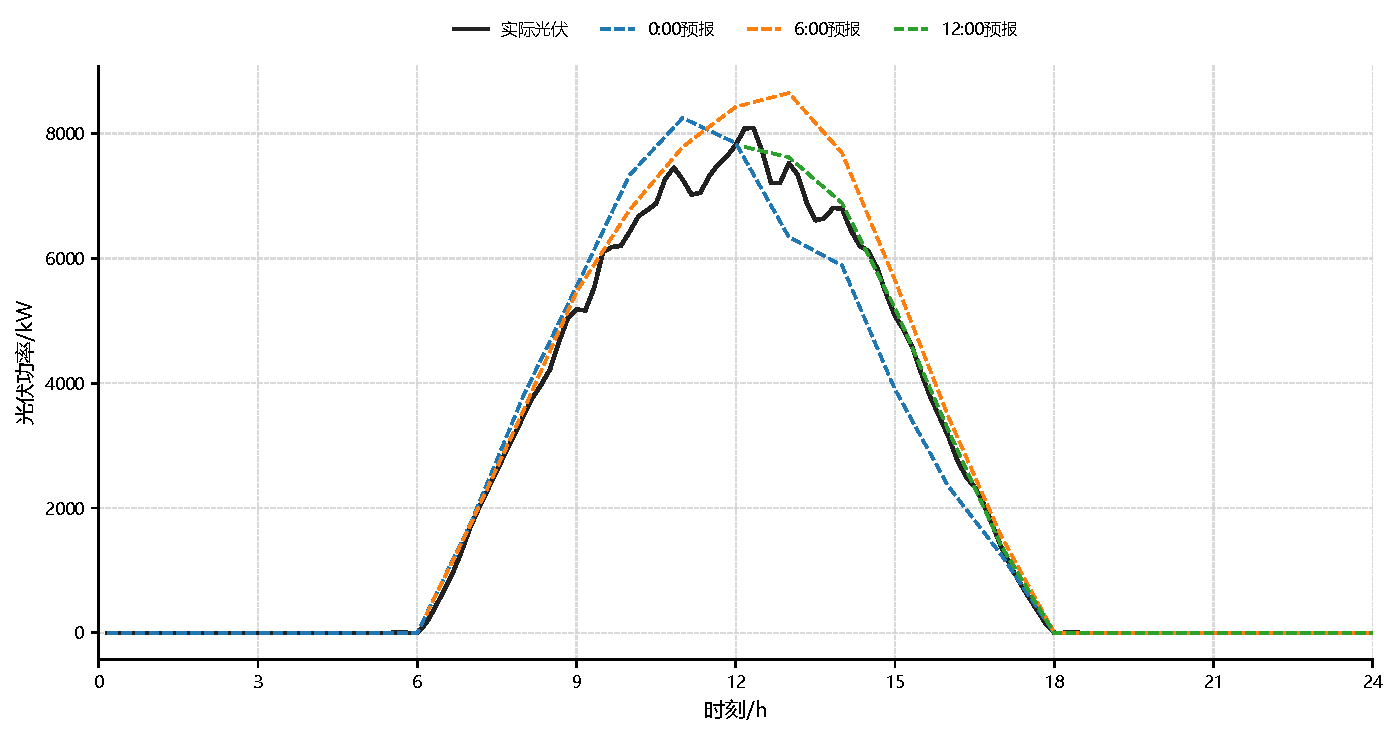
\includegraphics[width=0.72\textwidth]{../figures/问题三/问题三_指定日滚动光伏预报对比.pdf}
  \caption{2025 年 3 月 20 日各发布时点光伏预报与实际光伏对比}
  \label{fig:q3_day_pv}
\end{figure}

该日的滚动调度结果如图~\ref{fig:q3_day_sched} 所示：储能设备在午间低价时段充电、傍晚高价时段放电，实际紧急购电集中在凌晨与傍晚的少数时段。

\begin{figure}[H]
  \centering
  
\includegraphics[width=0.72\textwidth]{../figures/问题三/问题三_指定日滚动调度结果.pdf}
  \caption{2025 年 3 月 20 日滚动调度结果}
  \label{fig:q3_day_sched}
\end{figure}
